\section{Auswertung}
Die Auswertung, genauer die Fehlerrechnung, die Plots und Ausgleichsrechnung erfolgt mit den Paketen
Numpy \cite{numpy}, Uncertainties \cite{uncertainties}, Matplotlib \cite{matplotlib} und Scipy \cite{scipy} in der Programmiersprache python.
\subsection{Fehlerrechnung}
Der Mittelwert der Brechzahlen wird im Folgenden nach
\begin{equation}
  \bar{n}=\frac{1}{a}\sum_{i=1}^{a}n_i
\end{equation}
und sein Fehler mit
\begin{equation}
  \sigma_{\bar{n}}=\sqrt{\frac{1}{a(a-1)}\sum_{i=1}^{a}(\bar{n}-n_i)^2}
\end{equation}
gebildet.
\subsection{Kontrastmessung}
Vor Beginn der weiteren Auswertung muss zunächst der maximale Kontrast ermittelt werden.
Wie in der Durchführung beschrieben, wurde für die Messung vorgegangen; die Ergebnisse befinden sich in Tabelle $\ref{tab:kontrast}$.
Aus den gemessenen Extrema wurde nach Formel $\ref{eq:kontrast}$ der Kontrast berechnet.
Abbildung $\ref{fig:kontrastplot}$ enthält die graphische Darstellung der Kontrastmesswerte.
Erwartet wird ein Kontrast
\begin{equation}
  K \propto a|\cos(\phi)\sin(\phi)|.
\end{equation}
Infolgedessen wird eine Regression der Form
\begin{equation}
  K = a|\cos(\phi)\sin(\phi)|
\end{equation}
erstellt. Der Parameter $a$ ergib sich aus der Regression zu
\begin{equation*}
  a = 1,71 \pm 0,07.
\end{equation*}
Der maximale Kontrast folgt aus der Theoriekurve zu $K_\text{max}=0,86$.
Aus der Tabelle und dem Graphen ist zu entnehmen, dass die erwarteten Kontrastmaxima bei den erwarteten Stellen $45° , 135° , 225° \, \text{und} \, 315°$ zu finden sind.
Der Wert bei $\phi = 310°$ liegt dennoch höher als die anderen, sodass für die weiteren Messung mit eben dieser Einstellung weitergearbeitet wurde.
\begin{table}[H]
\centering
\begin{tabular}{c|c|c|c}
{$\phi \:/\: \textdegree$} & {$U_\text{max} \:/\: \si{mV}$} & {$U_\text{min} \:/\: \si{mV}$} & {$K$}\\
\midrule
0 & 1394 & 1181 & 0,08 \\
10 & 1194 & 769 & 0,22 \\
20 & 869 & 319 & 0,46 \\
30 & 744 & 175 & 0,62 \\
40 & 781 & 94 & 0,79 \\
50 & 913 & 56 & 0,88 \\
60 & 744 & 90 & 0,78 \\
70 & 919 & 131 & 0,75 \\
80 & 1147 & 469 & 0,42 \\
90 & 963 & 650 & 0,19 \\
110 & 2250 & 344 & 0,74 \\
130 & 1250 & 237 & 0,68 \\
150 & 2156 & 375 & 0,70 \\
170 & 1594 & 813 & 0,32 \\
190 & 1013 & 619 & 0,24 \\
210 & 819 & 188 & 0,63 \\
230 & 1125 & 75 & 0,88 \\
250 & 1297 & 187 & 0,75 \\
270 & 1138 & 788 & 0,18 \\
290 & 2172 & 641 & 0,54 \\
310 & 3562 & 125 & 0,93 \\
330 & 1781 & 375 & 0,65 \\
350 & 1750 & 984 & 0,28 \\
\end{tabular}
\caption{Messwerte der Spannungsextrema der Kontrastmessung.}
\label{tab:kontrast}
\end{table}
\begin{figure}[H]
  \centering
  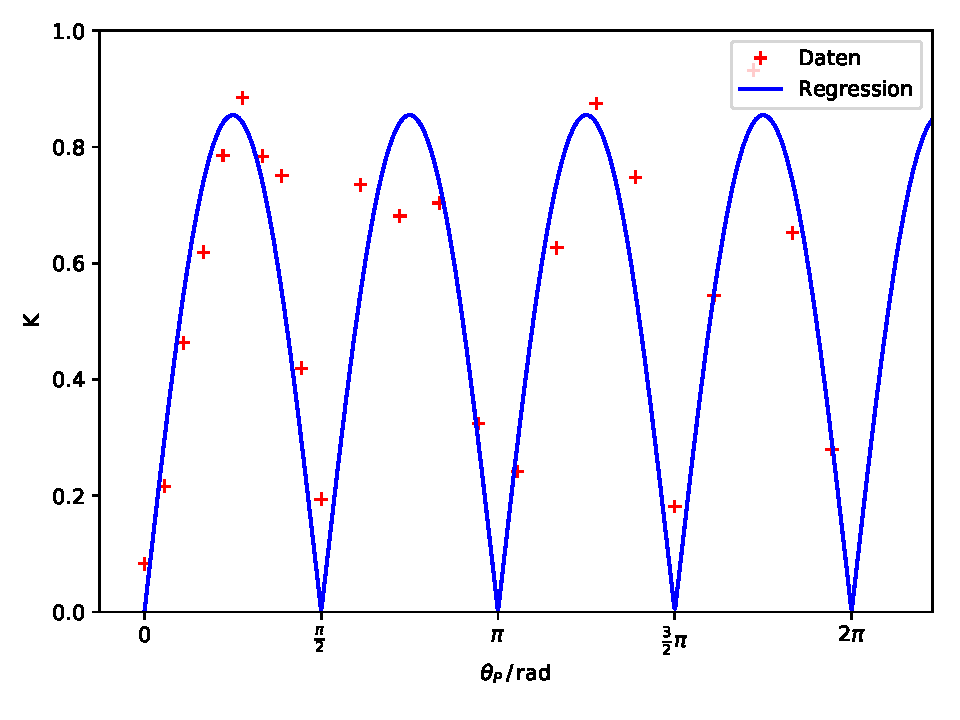
\includegraphics[scale=0.9]{bilder/kontrastplot.pdf}
  \caption{Graphische Darstellung der Kontrastmesswerte und Regression.}
  \label{fig:kontrastplot}
\end{figure}

\subsection{Brechungsindex der Glasplatten}
Durch das Drehen der Glasplatten soll, wie in der Durchführung beschrieben, über die bestimmten Intensitätsmaxima
der Brechungsindex $n$ berechnet werden.
Dies erfolgt nach Formel $\ref{eq:glas}$.
Als vom Hersteller gelieferte Angaben stehen die Dicke der Glasplättchen $T=\SI{1}{mm}$ und der Winkel der Platten zueinander $2\delta=20°$ zur Verfügung \cite{anleitung}.
Ein Theoriewert für den Brechungsindex ist durch $n= 1,45$ gegeben \cite{brechglas}.
Die Messung erfolgte über ein Intervall von $\theta = 10°$.
Tabelle $\ref{tab:glas}$ zeigt die Messwerte.

\begin{table}[H]
\centering
\begin{tabular}{c c c}
{Messung} & {$M$} & {$n_\text{Glas}$} \\
\midrule
1 & 35 & 1,571 \\
2 & 35 & 1,571 \\
3 & 36 & 1,598 \\
4 & 34 & 1,546 \\
5 & 34 & 1,546 \\
\end{tabular}
\caption{Messwerte zur Bestimmung des Brechungsindexes der Glasplättchen.}
\label{tab:glas}
\end{table}
Der Mittelwert des Brechungindexes folgt zu $\overline{n_\text{Glas}}=1,566 \pm 0,043$.\\
Es ergibt sich eine Abweichung von $7,4 \%$ zum Theoriewert.

\subsection{Brechnungsindex von Luft}
Die Berechnung des Brechungsindexes von Luft erfolgte bei einer Umgebungstemperatur von $\SI{23,4}{°C}$ und bei einem Druck von $\SI{994}{mbar}$.
Der Startwert nach der Evakuierung lag bei $\SI{6}{mbar}$.
Die Länge der Gaskammer beträgt $\SI{0,1}{m}$.
Der Brechungsindex wird mit Formel $\ref{eq:gas}$ berechnet.
\begin{table}[H]
\centering
\begin{tabular}{c c c}
{Messung} & {$M$} & {$n_\text{Luft}$} \\
\midrule
1 & 57 & 1,000361 \\
2 & 44 & 1,000279 \\
3 & 45 & 1,000285 \\
4 & 44 & 1,000279 \\
5 & 49 & 1,000310 \\
\end{tabular}
\caption{Messwerte zur Bestimmung des Brechungsindexes von Luft.}
\label{tab:luft}
\end{table}
Der Mittelwert und seine Abweichung ist $\overline{n_\text{Luft}}= 1,000303 \pm 0,000016$.\\
Der Theoriewert ist mit $n=1,000263 \pm 0,000000023$ angegeben \cite{brechglas2}.\\
Berücksichtigt wurde der an diesem Tag vorhandene Normaldruck $994\, mbar$ und die Raumtemperatur zum Messzeitpunkt von $23,4°C$.
Eine prozentuale Abweichung liegt mit $0,001\%$ vor.
